

% Redefine Headings
\renewcommand{\thechapter}{Appendix}
\titleformat{\chapter}{\normalfont\bfseries\centering}{\thechapter}{.25cm}{\uppercasetitle}[]

\renewcommand{\thesection}{\thechapter\enspace\Alph{section}}
\titleformat{\section}{\normalfont\bfseries\justifyheading}{\thesection.}{6pt}{}[]

% Prevent auto-add to TOC. Have to manually add to look nice.
\newcommand{\nocontentsline}[3]{}
\newcommand{\tocless}[2]{\bgroup\let\addcontentsline=\nocontentsline#1{#2}\egroup}
\addtocontents{toc}{\protect\setcounter{tocdepth}{1}}


\chapter*{APPENDICES} \label{appendix}
\addcontentsline{toc}{chapter}{Appendices}

\setcounter{section}{0}
\setcounter{appxcounter}{0}

\pagebreak
\tocless\section{Environment Data Structures} \label{sec:environment_data_structures}
\addcontentsline{toc}{section}{\thesection. Environment Data Structures}
This appendix contains all data structures related to an environment.
Together these traits, classes, and instances can be combined in different ways to create unique models of real-world environments.

\stepcounter{appxcounter}
\begin{appxlst}
  \caption{A class for representing a real-world environment. It is laid out in a grid of cells that contain information related to each of their respective areas within the grid.}
  \lstinputlisting{Codes/Environment.scala} \label{appendix:environment_class}
\end{appxlst}


\stepcounter{appxcounter}
\begin{appxlst}
  \caption{A class that represents a sub-section of an environment. The data stored in each instance represents the features that are found within the \texttt{Cell}'s area within the environment.}
  \lstinputlisting{Codes/Cell.scala} \label{appendix:cell_class}
\end{appxlst}


\stepcounter{appxcounter}
\begin{appxlst}
  \caption{An \texttt{Element} trait is a generalized representation of a measurable feature type within an environment. Specific element types can be created by extending this trait. Each instance defines specific information about what values can be represented for the specific element type.}
  \lstinputlisting{Codes/Element.scala} \label{appendix:elelment_trait}
\end{appxlst}


\stepcounter{appxcounter}
\begin{appxlst}
  \caption{\texttt{Elevation} is a class which extends the \texttt{Element} trait. This class models elevation levels within an environment. Different instances can be created to specify a level of elevation for each cell in an environment.}
  \lstinputlisting{Codes/Elevation.scala} \label{appendix:elevation_class}
\end{appxlst}


\stepcounter{appxcounter}
\begin{appxlst}
  \caption{An \texttt{Anomaly} is any object within an environment that may be of interest. Anomalies often have a set of effects that will alter the environment around them. This trait can be extended to define specific types of anomalies that can be represented in an environment.}
  \lstinputlisting{Codes/Anomaly.scala} \label{appendix:anomaly_trait}
\end{appxlst}

\stepcounter{appxcounter}
\begin{appxlst}
  \caption{The \texttt{Effect} trait is a generalized description of an alteration that an \texttt{Anomaly} has on the environment. Effects will alter a single element type in an area of the environment that the anomaly is located within.}
  \lstinputlisting{Codes/Effect.scala} \label{appendix:effect_trait}
\end{appxlst}

\stepcounter{appxcounter}
\begin{appxlst}
  \caption{\texttt{Human} is a specific \texttt{Anomaly} class. This class represents a peron that could be found in an environment. Human's have two defined \texttt{Effects}: sound and heat. These effects will alter the decibel and temperature element values in the human's general area within the environment.}
  \lstinputlisting{Codes/Human.scala} \label{appendix:human_class}
\end{appxlst}

\stepcounter{appxcounter}
\begin{appxlst}
  \caption{A \texttt{Layer} holds a collection of instances of a specific \texttt{Element} class. The collection is represented as a 2-dimentional grid that is relative to an \texttt{Environment} grid. They can be thought of as the same structure as an environment, but only containing information about a single element type.}
  \lstinputlisting{Codes/Layer.scala} \label{appendix:layer_class}
\end{appxlst}





\pagebreak
\tocless\section{Agent Data Structures} \label{sec:agent_data_structres}
\addcontentsline{toc}{section}{\thesection. Agent Data Structures}
This appendix contains data structures that are representative of an agent.
These structures model the different capabilities an agent has to interact with an environment.


\stepcounter{appxcounter}
\begin{appxlst}
  \caption{An \texttt{Agent} represents a physical member capable of acting within an environment. The class defines a controller for selecting actions, sensors that the agent is equipped with, mobility and durability features of the agent for modeling interactions with an environment, and several internal status variables.}
  \lstinputlisting{Codes/Agent.scala} \label{appendix:agent_class}
\end{appxlst}


\stepcounter{appxcounter}
\begin{appxlst}
  \caption{A \texttt{Sensor} is a tool that an agent can utilize to collect data about a specific element type within an environment. Sensors have a set range and energy cost related to using them.}
  \lstinputlisting{Codes/Sensor.scala} \label{appendix:sensor_class}
\end{appxlst}


\stepcounter{appxcounter}
\begin{appxlst}
  \caption{\texttt{Mobility} contains a set of variables related to how an agent will be able to safely move within an environment.}
  \lstinputlisting{Codes/Mobility.scala} \label{appendix:mobility_class}
\end{appxlst}


\stepcounter{appxcounter}
\begin{appxlst}
  \caption{\texttt{Durability} defines how an agent will interact with an element type in an environment. Different agents will each have strengths and weaknesses defined by how they will react when in contact with certain elements in an environment.}
  \lstinputlisting{Codes/Durability.scala} \label{appendix:durability_class}
\end{appxlst}


\stepcounter{appxcounter}
\begin{appxlst}
  \caption{An \texttt{AgentState} represents an instance of the internal status of an agent and the information that the agent knows about its environment. An \texttt{Agent}'s internal map is condensed into a set of sub-states within the entire agent state for each element type that the agent has knowledge of.}
  \lstinputlisting{Codes/AgentState.scala} \label{appendix:agentstate_class}
\end{appxlst}


\stepcounter{appxcounter}
\begin{appxlst}
  \caption{\texttt{ElementState}s are representative of an agent's knowledge of a specific element type in an environment. The information contained is directly related to what the agent has gathered into its internal map through the use a sensor. Specific known values of the element type are divided into four quadrants relative to the agent's current position.}
  \lstinputlisting{Codes/ElementState.scala} \label{appendix:elementstate_class}
\stepcounter{appxcounter}
\end{appxlst}


\stepcounter{appxcounter}
\begin{appxlst}
  \caption{A \texttt{QuadrantState} represents a collection of known information about a specific element type in a sub-set of cells within an environment. The data is condensed to an average known value differential and immediate known value differential relative to the value in the cell that the agent currently occupies.}
  \lstinputlisting{Codes/QuadrantState.scala} \label{appendix:quadrantstate_class}
\end{appxlst}


\stepcounter{appxcounter}
\begin{appxlst}
  \caption{\texttt{Controller}s are the decision-making models that are used to select actions for an agent to take. The process that each controller uses to select an action vary, but must choose from a set of valid actions and can use information that the agent has gathered while exploring the environment.}
  \lstinputlisting{Codes/Controller.scala} \label{appendix:controller_trait}
\end{appxlst}





\pagebreak
\tocless\section{Environment Generation Data Structures} \label{sec:environment_generation_data_structures}
\addcontentsline{toc}{section}{\thesection. Environment Generation Data Structures}
This appendix includes the data structures used to guide the procedural generation of unique environments.

\stepcounter{appxcounter}
\begin{appxlst}
  \caption{\texttt{EnvironmentTemplate}s hold the entire collection of attributes that are used to guide the process of generating an environment.}
\lstinputlisting{Codes/EnvironmentTemplate.scala} \label{appendix:environmenttemplate_class}
\end{appxlst}


\stepcounter{appxcounter}
\begin{appxlst}
  \caption{\texttt{ElementSeed} is a trait used to define helper classes for specific \texttt{Element} classes. They have a set of attributes that can be set to guide how the element type will be initialized in an environment and functions related to the actual process in which the element type will be procedurally generated within the environment.}
\lstinputlisting{Codes/ElementSeed.scala} \label{appendix:elementseed_trait}
\end{appxlst}


\stepcounter{appxcounter}
\begin{appxlst}
  \caption{A \texttt{TerrainModification} is a trait used for defining processes to alter element types within the environment. These help to add unique features within element types found in the environment.}
\lstinputlisting{Codes/TerrainModification.scala} \label{appendix:terrainmodification_trait}
\end{appxlst}





\pagebreak
\tocless\section{State Comparison Data Structures} \label{sec:state_comparison_data_structures}
\addcontentsline{toc}{section}{\thesection. State Comparison Data Structures}
This appendix includes data structures related to comparing multiple \texttt{AgentState}s to each other.

\stepcounter{appxcounter}
\begin{appxlst}
  \caption{\texttt{GaussianData} holds the mean and standard deviation of a collection of values.}
\lstinputlisting{Codes/GaussianData.scala} \label{appendix:gaussian_data}
\end{appxlst}


\stepcounter{appxcounter}
\begin{appxlst}
  \caption{\texttt{StateActionDifference} holds values related to a comparison that was made between a current \texttt{AgentState} and an \texttt{AgentState} within SCOUt's memory of state-action rewards. Each instance defines the differences that were calculated between two states, an overall state difference, the action that was taken by the agent in the state-action reward, and then the short-term and long-term rewards that the were received for the action.}
\lstinputlisting{Codes/StateActionDifference.scala} \label{appendix:state_action_difference}
\end{appxlst}








\pagebreak
\tocless\section{Experimentation Setup} \label{sec:experiment_setup}
\addcontentsline{toc}{section}{\thesection. Experimentation Setup}
This appendix includes the code listings for the \texttt{Agent} configuration and \texttt{EnvironmentTemplate}s used in experimentation.

\stepcounter{appxcounter}
\begin{appxlst}
  \caption{Instances of the \texttt{Agent} class and \texttt{Sensor} classes that are used in experimentation. Some attributes are set per operation during experiments. These are marked with a comment ``Defined Per Operation.''}
  \lstinputlisting[linerange={1-34}]{Codes/TestAgentSetup.scala} \label{appendix:agent_setup}
\end{appxlst}
\begin{appxlst}
  \caption{...Continued}
  \lstinputlisting[linerange={34-68},firstnumber=34]{Codes/TestAgentSetup.scala} \label{appendix:agent_setup}
\end{appxlst}


\stepcounter{appxcounter}
\begin{appxlst}
  \caption{JSON data storing the an environment template used in experimentation. This template is title \textit{EASY} as it represents a relatively easy environment for an operation to take place in. The environment is $8\times8$ cells and contains only one modification for a pool of water to be generated within the environment.}
  \lstinputlisting[language=Java,linerange={0-40}]{Codes/EASY.json} \label{appendix:easy_environmenttemplate}
\end{appxlst}
\begin{appxlst}
  \caption{...Continued}
  \lstinputlisting[language=Java,linerange={41-85},firstnumber=41]{Codes/EASY.json} \label{appendix:easy_environmenttemplate}
\end{appxlst}


\stepcounter{appxcounter}
\begin{appxlst}
  \caption{JSON data storing the an environment template used in experimentation. This template is title \textit{MEDIUM} as it presents a few challenging features that an agent may face. The environment is $10\times10$ cells and contains both a ``hill'' elevation modification and a water pool modification. Compared to the \textit{EASY} environment template, \textit{MEDIUM} has higher ambient levels of decibel and temperature values, making it slightly more difficult to identify the effects of a human anomaly within the environment.}
  \lstinputlisting[language=Java,linerange={0-38}]{Codes/MEDIUM.json} \label{appendix:medium_environmenttemplate}
\end{appxlst}
\begin{appxlst}
  \caption{...Continued}
  \lstinputlisting[language=Java,linerange={39-81},firstnumber=39]{Codes/MEDIUM.json} \label{appendix:medium_environmenttemplate}
\end{appxlst}
\begin{appxlst}
  \caption{...Continued}
  \lstinputlisting[language=Java,linerange={82-101},firstnumber=82]{Codes/MEDIUM.json} \label{appendix:medium_environmenttemplate}
\end{appxlst}



\stepcounter{appxcounter}
\begin{appxlst}
  \caption{JSON data storing the an environment template used in experimentation. This template is title \textit{HARD} as it presents many challenging features that an agent may face. The environment is $12\times12$ cells and contains a ``hill'' elevation modification, a ``valley'' elevation modification, a water pool modification, and a water stream modification. Additionally, the ambient levels of decibel values and temperature values are raised and the sound and heat effects of the human anomaly are suppressed even more than seen in the \textit{MEDIUM} environment template. The combination of all of these factors create environments that are both highly difficult to safely navigate and difficult to identify anomaly effects within.}
  \lstinputlisting[language=Java,linerange={0-36}]{Codes/HARD.json} \label{appendix:hard_environmenttemplate}
\end{appxlst}
\begin{appxlst}
  \caption{...Continued}
  \lstinputlisting[language=Java,linerange={37-79},firstnumber=37]{Codes/HARD.json} \label{appendix:hard_environmenttemplate}
\end{appxlst}
\begin{appxlst}
  \caption{...Continued}
  \lstinputlisting[language=Java,linerange={80-122},firstnumber=80]{Codes/HARD.json} \label{appendix:hard_environmenttemplate}
\end{appxlst}
\begin{appxlst}
  \caption{...Continued}
  \lstinputlisting[language=Java,linerange={123-139},firstnumber=123]{Codes/HARD.json} \label{appendix:hard_environmenttemplate}
\end{appxlst}





\pagebreak
\tocless\section{Training Variation 1} \label{sec:training_variation1}
\addcontentsline{toc}{section}{\thesection. Training Variation 1}
This appendix contains results for our first variation of training the three SCOUt controller memories ($SCOUt_{FH}$, $SCOUt_{MW}$, and $SCOUt_{H}$).
During training and iteration testing, the long-term reward (algorithm~\ref{algorithmic:long_term_reward}) was adjusted to only factor in a \texttt{goalReward} if the agent had remaining health at the end of an operation.
This was done to observe how SCOUt controllers would change the agent's behavior when their memory of state-action rewards reflected smaller long-term rewards from operations where the agent's health was depleted.
It was hoped that we would see better performance in average remaining energy and subsequently all other areas.
However, we found no significant improvements in performance.
Appendix~\ref{appendix:findhuman_training_variation1} shows the results for $SCOUt_{FH}$, Appendix~\ref{appendix:mapwater_training_variation1} shows the results for $SCOUt_{MW}$, and Appendix~\ref{appendix:hybrid_training_fh_variation1} and~\ref{appendix:hybrid_training_mw_variation1} show results for $SCOUt_{H}$ in \textit{Find Human} and \textit{Map Water} operations, respectively.

\stepcounter{appxcounter}
\begin{appxfig}[H]
\begin{figure}[H]
  \centering
  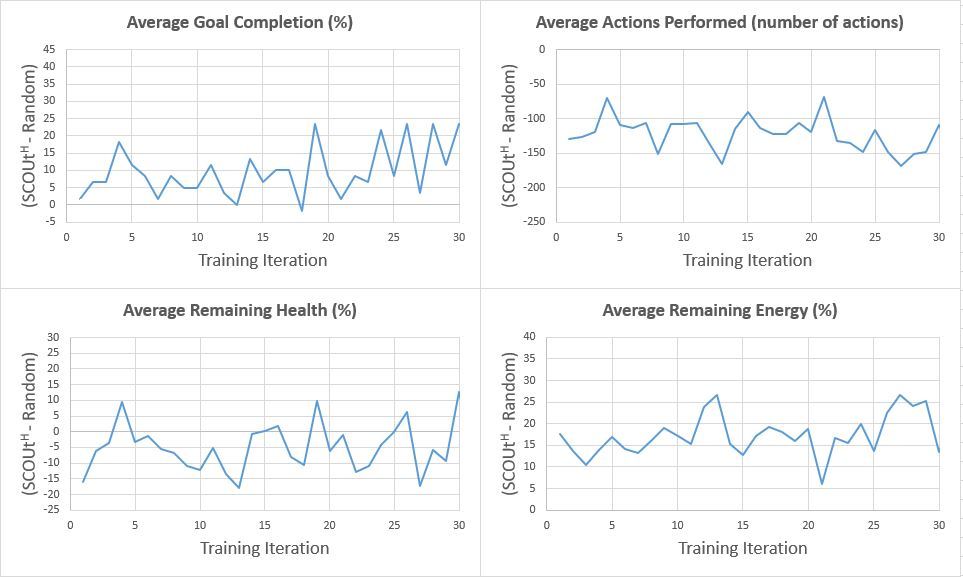
\includegraphics[width=0.9\columnwidth]{Figures/Results/TrainingVariation1/FindHuman.JPG}
\end{figure}
\caption{Iteration testing performance results for $SCOUt_{FH}$ attempting \textit{Find Human} using setup variation 1 (see subsection~\ref{subsec:training_variations}). All graphs show the controller's average difference in performance compared to $Random$ ($SCOUt_{FH}$ average - $Random$ average) VS the number of training iterations completed.}
\label{appendix:findhuman_training_variation1}
\end{appxfig}


\stepcounter{appxcounter}
\begin{appxfig}[H]
\begin{figure}[H]
  \centering
  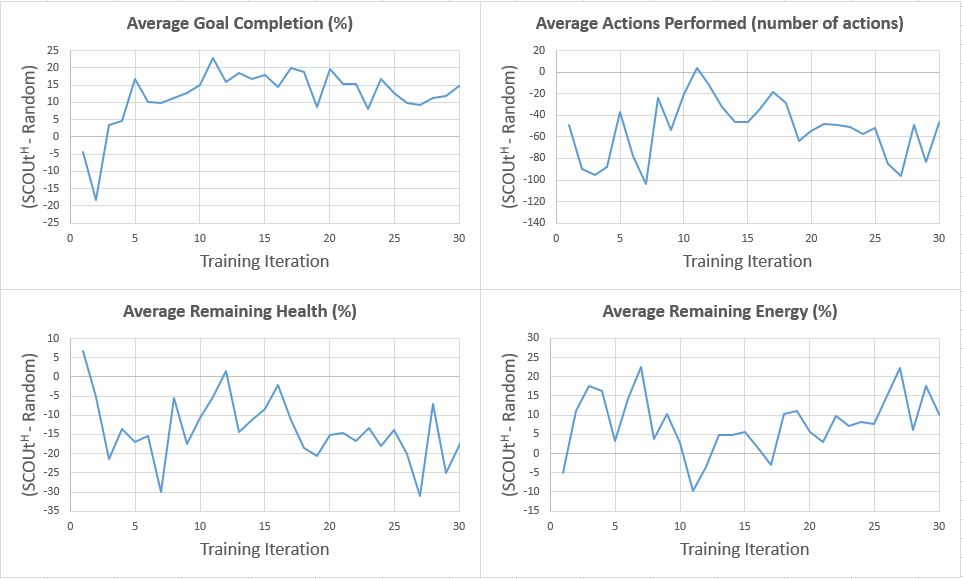
\includegraphics[width=0.9\columnwidth]{Figures/Results/TrainingVariation1/MapWater.JPG}
\end{figure}
\caption{Iteration testing performance results for $SCOUt_{MW}$ attempting \textit{Map Water} using setup variation 1 (see subsection~\ref{subsec:training_variations}). All graphs show the controller's average difference in performance compared to $Random$ ($SCOUt_{MW}$ average - $Random$ average) VS the number of training iterations completed.}
\label{appendix:mapwater_training_variation1}
\end{appxfig}


\stepcounter{appxcounter}
\begin{appxfig}[H]
\begin{figure}[H]
  \centering
  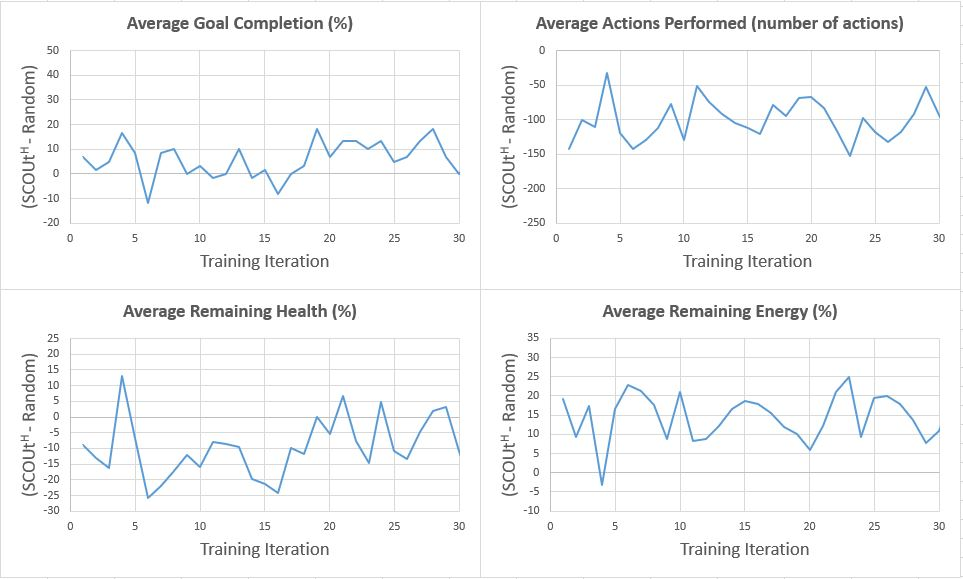
\includegraphics[width=0.9\columnwidth]{Figures/Results/TrainingVariation1/Hybrid-FindHuman.JPG}
\end{figure}
\caption{Iteration testing performance results for $SCOUt_{H}$ attempting \textit{Find Human} using setup variation 1 (see subsection~\ref{subsec:training_variations}). All graphs show the controller's average difference in performance compared to $Random$ ($SCOUt_{H}$ average - $Random$ average) VS the number of training iterations completed.}
\label{appendix:hybrid_training_fh_variation1}
\end{appxfig}


\stepcounter{appxcounter}
\begin{appxfig}[H]
\begin{figure}[H]
  \centering
  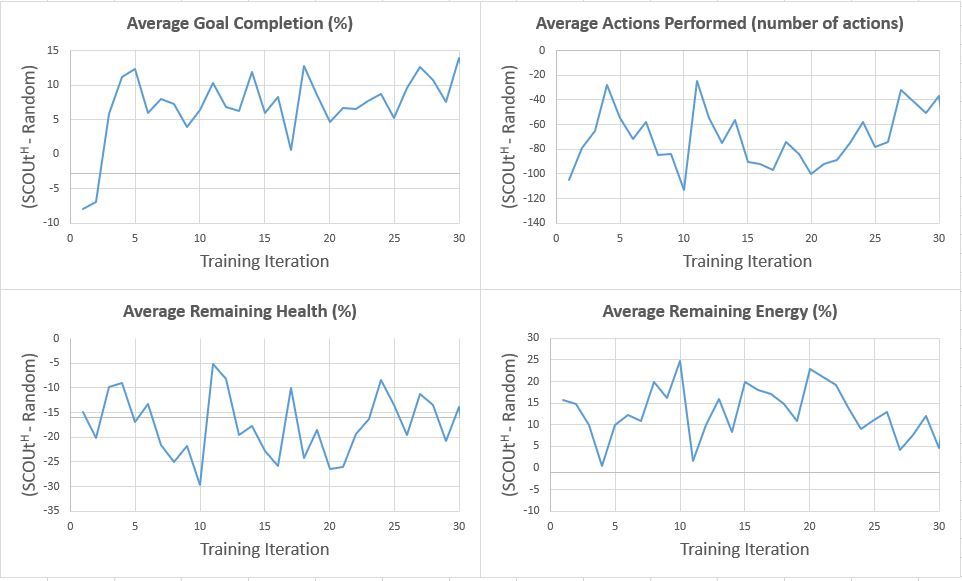
\includegraphics[width=0.9\columnwidth]{Figures/Results/TrainingVariation1/Hybrid-MapWater.JPG}
\end{figure}
\caption{Iteration testing performance results for $SCOUt_{H}$ attempting \textit{Map Water} using setup variation 1 (see subsection~\ref{subsec:training_variations}). All graphs show the controller's average difference in performance compared to $Random$ ($SCOUt_{H}$ average - $Random$ average) VS the number of training iterations completed.}
\label{appendix:hybrid_training_mw_variation1}
\end{appxfig}







\pagebreak
\tocless\section{Training Variation 2} \label{sec:training_variation2}
\addcontentsline{toc}{section}{\thesection. Training Variation 2}
This appendix contains results for our second variation of training the three SCOUt controller memories ($SCOUt_{FH}$, $SCOUt_{MW}$, and $SCOUt_{H}$).
During training and iteration testing, the \textit{goalRewardWeight} used for calculating long-term reward (algorithm~\ref{algorithmic:long_term_reward}) was set to 1.5.
This was done to observe how SCOUt controllers would change the agent's behavior when their memory of state-action rewards reflected a stronger emphasis on the level of goal completion attained.
It was hoped that we would see better performance in all categories.
While only slight improvements were observed, this method was chosen for all testing conducted in our experimentation.
Appendix~\ref{appendix:findhuman_training_variation2} shows the results for $SCOUt_{FH}$, Appendix~\ref{appendix:mapwater_training_variation2} shows the results for $SCOUt_{MW}$, and Appendix~\ref{appendix:hybrid_training_fh_variation2} and~\ref{appendix:hybrid_training_mw_variation2} show results for $SCOUt_{H}$ in \textit{Find Human} and \textit{Map Water} operations, respectively.

\stepcounter{appxcounter}
\begin{appxfig}[H]
\begin{figure}[H]
  \centering
  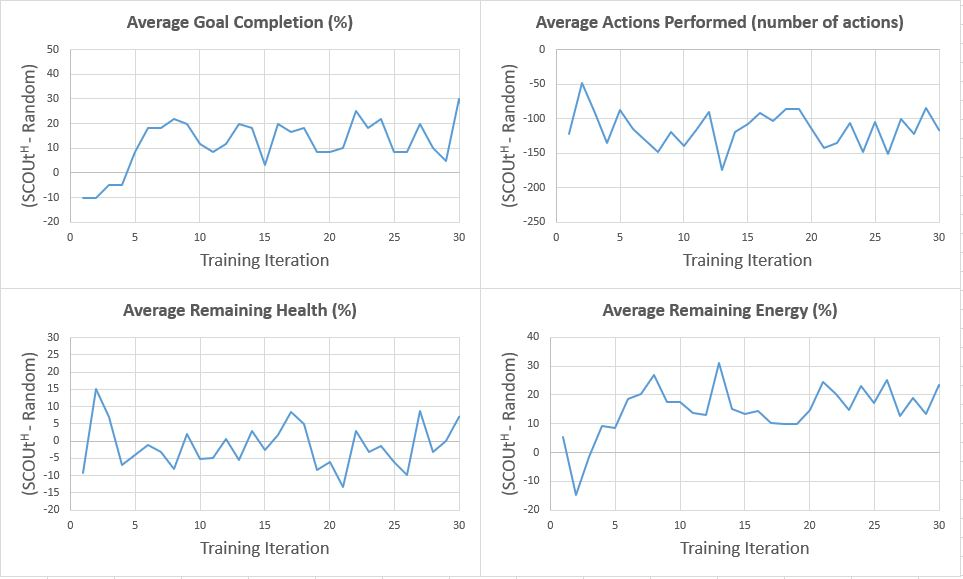
\includegraphics[width=0.9\columnwidth]{Figures/Results/TrainingVariation2/FindHuman.JPG}
\end{figure}
\caption{Iteration testing performance results for $SCOUt_{FH}$ attempting \textit{Find Human} using setup variation 2 (see subsection~\ref{subsec:training_variations}). All graphs show the controller's average difference in performance compared to $Random$ ($SCOUt_{FH}$ average - $Random$ average) VS the number of training iterations completed.}
\label{appendix:findhuman_training_variation2}
\end{appxfig}


\stepcounter{appxcounter}
\begin{appxfig}[H]
\begin{figure}[H]
  \centering
  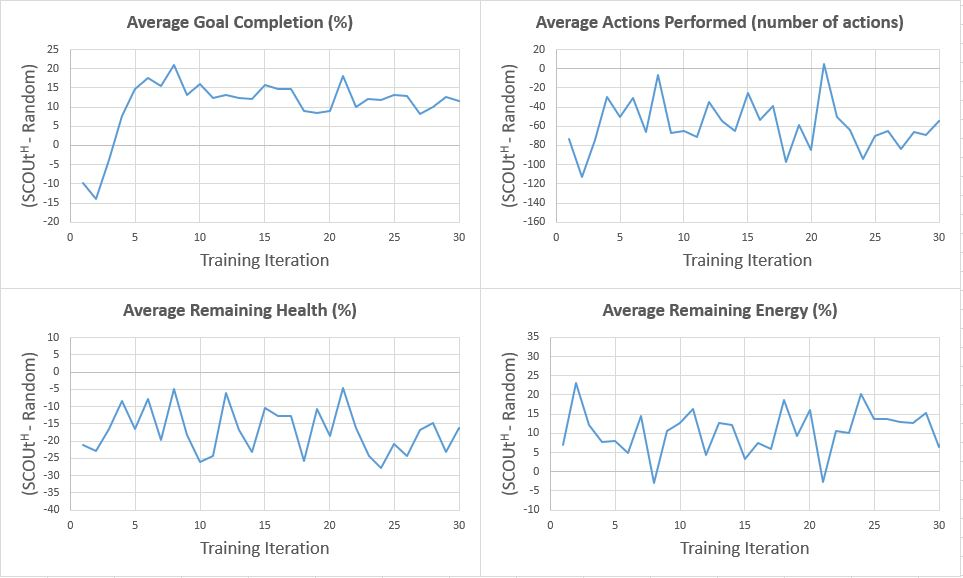
\includegraphics[width=0.9\columnwidth]{Figures/Results/TrainingVariation2/MapWater.JPG}
\end{figure}
\caption{Iteration testing performance results for $SCOUt_{MW}$ attempting \textit{Map Water} using setup variation 2 (see subsection~\ref{subsec:training_variations}). All graphs show the controller's average difference in performance compared to $Random$ ($SCOUt_{MW}$ average - $Random$ average) VS the number of training iterations completed.}
\label{appendix:mapwater_training_variation2}
\end{appxfig}


\stepcounter{appxcounter}
\begin{appxfig}[H]
\begin{figure}[H]
  \centering
  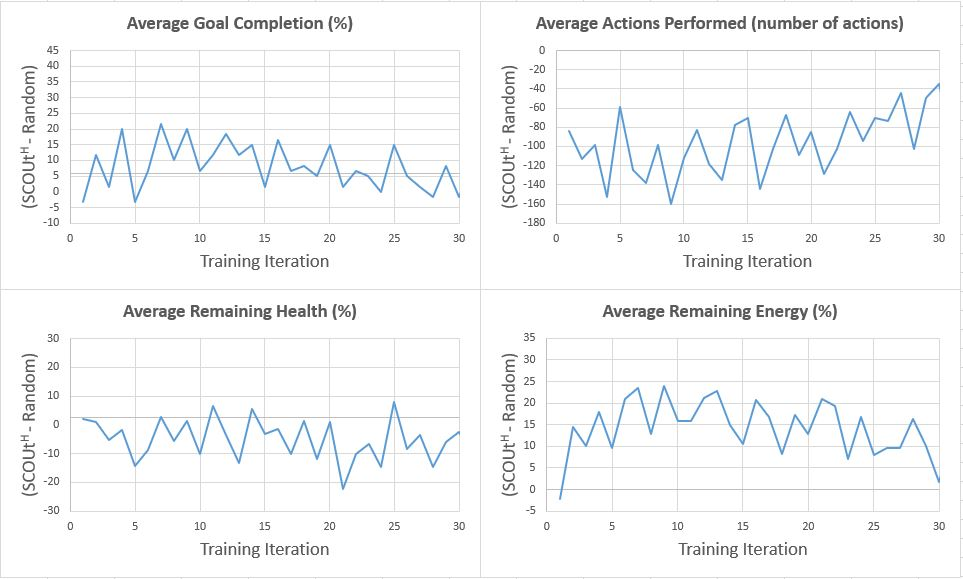
\includegraphics[width=0.9\columnwidth]{Figures/Results/TrainingVariation2/Hybrid-FindHuman.JPG}
\end{figure}
\caption{Iteration testing performance results for $SCOUt_{H}$ attempting \textit{Find Human} using setup variation 2 (see subsection~\ref{subsec:training_variations}). All graphs show the controller's average difference in performance compared to $Random$ ($SCOUt_{H}$ average - $Random$ average) VS the number of training iterations completed.}
\label{appendix:hybrid_training_fh_variation2}
\end{appxfig}


\stepcounter{appxcounter}
\begin{appxfig}[H]
\begin{figure}[H]
  \centering
  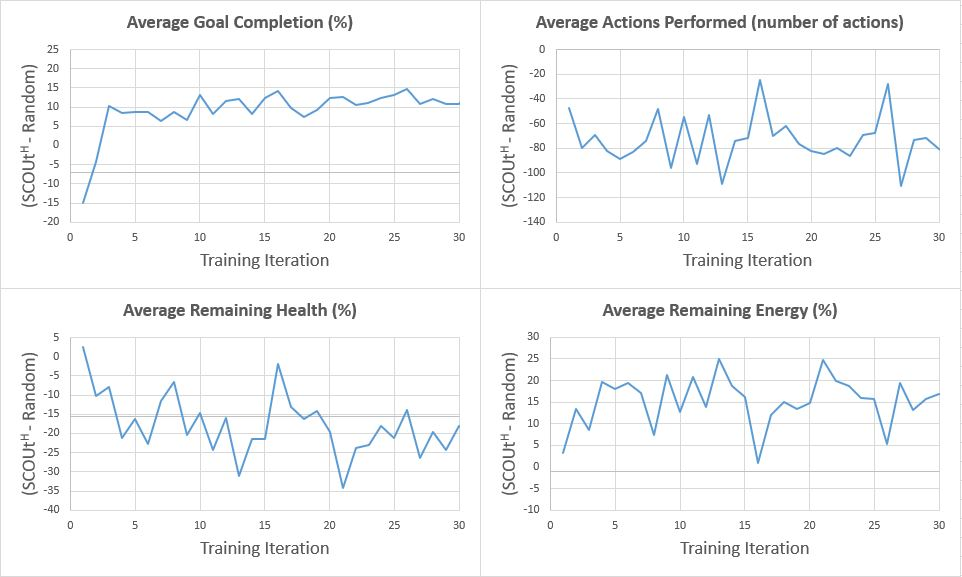
\includegraphics[width=0.9\columnwidth]{Figures/Results/TrainingVariation2/Hybrid-MapWater.JPG}
\end{figure}
\caption{Iteration testing performance results for $SCOUt_{H}$ attempting \textit{Map Water} using setup variation 2 (see subsection~\ref{subsec:training_variations}). All graphs show the controller's average difference in performance compared to $Random$ ($SCOUt_{H}$ average - $Random$ average) VS the number of training iterations completed.}
\label{appendix:hybrid_training_mw_variation2}
\end{appxfig}





%
% \tocless\section{Appendix C: Mathematical Proofs} \label{appendix:proofs}
% This appendix contains mathematical proofs related to the use of Gaussian normalization on value sets.
%
%
%
% \begin{algorithm}[H]
%   \setstretch{1.35}
%   \caption{Proof that...}
%   \begin{algorithmic} \label{appendix:gaussian_difference_identical}
%     \REQUIRE $mean \leftarrow 10$
%     \REQUIRE $sd \leftarrow 1$
%     \REQUIRE $x = y$
%     \ENSURE $x_{normal} = y_{normal}$
%     \STATE $x_{normal} \leftarrow (x - mean) / sd$
%     \STATE $x = y$
%     \STATE $x = y$
%     \STATE $x = y$
%     \STATE $x = y$
%     \STATE $x = y$
%
%   \end{algorithmic}
% \end{algorithm}
%
%
% \begin{lstlisting}[label=appendix:gaussian_difference_identical]
% Example:
% Gaussian mean = 10
% Gaussian standard deviation = 1
%
% x = 12
% y = 12
% x = y
%
% x(normalized) = (x - Gaussain mean) / Gaussian standard deviation
% x(normalized) = (12 - 10) / 1
% x(normalized) = 2 / 1
% x(normalized) = 2
%
% y(normalized) = (y - Gaussain mean) / Gaussian standard deviation
% y(normalized) = (12 - 10) / 1
% y(normalized) = 2 / 1
% y(normalized) = 2
%
% x(normalized) = y(normalized)
%
% Gaussian difference (x,y) = |x - y|
% Gaussian difference (x,y) = |2 - 2|
% Gaussian difference (x,y) = 0
% \end{lstlisting}
%
%
% \begin{lstlisting}[label=appendix:gaussian_difference_different]
% Example:
% Gaussian mean = 10
% Gaussian standard deviation = 1
%
% x = 12
% y = 7
%
% x(normalized) = (x - Gaussain mean) / Gaussian standard deviation
% x(normalized) = (12 - 10) / 1
% x(normalized) = 2 / 1
% x(normalized) = 2
%
% y(normalized) = (y - Gaussain mean) / Gaussian standard deviation
% y(normalized) = (7 - 10) / 1
% y(normalized) = -3 / 1
% y(normalized) = -3
%
% Gaussian difference (x,y) = |x - y|
% Gaussian difference (x,y) = |2 - -3|
% Gaussian difference (x,y) = 5
% \end{lstlisting}
